\section{Sea Surface Temperature and the Health of Phytoplankton}

To begin investigating what affects marine heat waves have on the health of phytoplankton, we must first establish what how sea surface temperature impact the health of phytoplankton as MHWs are periods of exceptionally high sea surface temperatures. To do these we will choose three locations that are covered by our SST and chlorophyll concentration data. To decide these locations we sought out areas that see a variety variance in SST through out the year and varied across water depth, using a location close to shore, very far from shore and in the middle. This will allow us to use the natural changes of SST due to seasonal changes as a way to vary temperature of the location whilst allowing us to keep other variables relatively constant.
\\\\
Using a variation of the R script used in "Heartbeat of the Southern Oscillation explains ENSO climatic resonances" \cite{bruun2017heartbeat} we will construct an ARIMA model as discussed in \autoref{subsec:ARIMA} for both the SST and chlorophyll concentration data time series. From these models we will create an annual climatology to take a deeper look into the relationship between SST and chlorophyll concentration.

\subsection{Climatology Plots: Indian Ocean}

We decided to use three points in the Indian Ocean just west of western Australia equally spaced by five degree's latitude.

\subsubsection{Close to the shore: -24$^{\circ}$N 113$^{\circ}$E}

This location is the closest to the Australian shore, at just over 25 miles. 

\begin{figure*}[h]
    \centering
    \begin{subfigure}[t]{0.5\textwidth}
        \centering
        \includegraphics[width=0.7\textwidth, angle =-90]{Chapter3/-24,113/Data_-24N113E_Chl_Climatology.eps}
    \end{subfigure}%
    ~ 
    \begin{subfigure}[t]{0.5\textwidth}
        \centering
        \includegraphics[width=0.7\textwidth, angle =-90]{Chapter3/-24,113/Data_-24N113E_SST_Climatology.eps}
    \end{subfigure}
    \caption{Two plots, one on the left of the annual climatology of chlorophyll concentration and on the right the annual climatology of sea surface temperature both at -24$^{\circ}$N 113$^{\circ}$E.}\label{fig:clim-24,113}
\end{figure*}

\pagebreak

\subsubsection{Far from the shore: -24$^{\circ}$N 108$^{\circ}$E}

This location is the next closest to the Australian shore, being 350 miles away. 

\begin{figure*}[ht]
    \centering
    \begin{subfigure}[t]{0.5\textwidth}
        \centering
        \includegraphics[width=0.7\textwidth, angle =-90]{Chapter3/-24,108/Data_-24N108E_Chl_Climatology.eps}
    \end{subfigure}%
    ~ 
    \begin{subfigure}[t]{0.5\textwidth}
        \centering
        \includegraphics[width=0.7\textwidth, angle =-90]{Chapter3/-24,108/Data_-24N108E_SST_Climatology.eps}
    \end{subfigure}
    \caption{Two plots, one on the left of the annual climatology of chlorophyll concentration and on the right the annual climatology of sea surface temperature -24$^{\circ}$N 108$^{\circ}$E.}\label{fig:clim-24,108}
\end{figure*}

\subsubsection{Deep ocean -24$^{\circ}$N 103$^{\circ}$E}

This location is in the deep Indian ocean, being over 650 miles from the closest shore. 

\begin{figure*}[ht]
    \centering
    \begin{subfigure}[t]{0.5\textwidth}
        \centering
        \includegraphics[width=0.7\textwidth, angle =-90]{Chapter3/-24,103/Data_-24N103E_Chl_Climatology.eps}
    \end{subfigure}%
    ~ 
    \begin{subfigure}[t]{0.5\textwidth}
        \centering
        \includegraphics[width=0.7\textwidth, angle =-90]{Chapter3/-24,103/Data_-24N103E_SST_Climatology.eps}
    \end{subfigure}
    \caption{Two plots, one on the left of the annual climatology of chlorophyll concentration and on the right the annual climatology of sea surface temperature -24$^{\circ}$N 103$^{\circ}$E.}\label{fig:clim-24,103}
\end{figure*}

\subsection{Analysing the Climatology Plots}

Firstly looking at \autoref{fig:clim-24,113}, we see that the two plots indicate that there is a inverse relationship between the two variables, SST and chlorophyll concentration. This is seen by the periods (months) where chlorophyll concentration is the lowest, the SST climatology plot is at the highest. Then as sea surface temperature starts to decrease (around month 4) we begin to see an increase in chlorophyll concentration. Chlorophyll concentration again starts to decrease (around month 8) SST starts to increase again around one month later. It is worth noting that the range off the SST data at -24$^{\circ}$N 113$^{\circ}$E is considerable larger than the other locations, this is due to coastal areas generally showing fluctuations in water temperature closely paralleled to air temperature \cite{LALLI199716} due to an easy transfer of thermal energy between the shallow water and atmosphere.
\\\\
Now looking at \autoref{fig:clim-24,108} and \autoref{fig:clim-24,103} we see a much more complicated SST climatology plot and also over a much smaller range of temperatures. These two figures do not inversely relate as well as in \autoref{fig:clim-24,113} but still indicate a inverse relationship between the two variable. Despite the differences in the shape of the SST climatology plots, all three locations have similar shaped chlorophyll concentration plots, with their range from minimum and maximum values appearing to be scaled proportionally by the range of their corresponding SST climatology plot. All three chlorophyll concentration plots see a sharp increase in month four (April) which is the second month into autumn, just two months before winter when Western Australia sees it's coldest temperatures. It then reaches a peak around month 8 (August) before taking a sharp decline, this is shortly before summer, the season with highest temperature. These plots hence hint at a negative correlation between SST and chlorophyll concentration but also show that there are other factors that play a role.

\subsection{Regression Analysis}

In this section we will be using our data used to produce our climatology plots in a scatter plot and use the R function "abline" to calculate and plot a regression line.

\begin{figure*}[ht]
    \centering
    \begin{subfigure}[t]{0.5\textwidth}
        \centering
        \includegraphics[width=0.7\textwidth, angle =-90]{Chapter3/-24,103/Data_-24N103E_Regression.eps}
    \end{subfigure}%
    ~
    \begin{subfigure}[t]{0.5\textwidth}
        \centering
        \includegraphics[width=0.7\textwidth, angle =-90]{Chapter3/-24,108/Data_-24N108E_Regression.eps}
    \end{subfigure}
    ~
    \begin{subfigure}[t]{0.5\textwidth}
    \centering
    \includegraphics[width=0.7\textwidth, angle =-90]{Chapter3/-24,103/Data_-24N103E_Regression.eps}
    \end{subfigure}
    \caption{Chlorophyll concentration plotted against sea surface temperature for three different locations in the Indian Ocean. From top left to right: -24$^{\circ}$N 113$^{\circ}$E, -24$^{\circ}$N 108$^{\circ}$E, -24$^{\circ}$N 103$^{\circ}$E}.\label{fig:reg}
\end{figure*}

\noindent As indicated in the previous section, from our data set there is a negative correlation between chlorophyll concentration and SST. Whilst the temperature of the water will affect both the biological and chemical processes for aquatic systems. It has been shown in literature that the nutrient suppressing effects of increased SST suppresses the temperature dependence of metabolic rates \cite{maranon2018nutrient}. 

\subsubsection{Nutrient suppression from increased sea surface temperature}

Phytoplankton are crucially dependent on nutrients. These are primarily macro-nutrients such as nitrate, phosphate or silicic acid, whose availability is governed by the balance between the so-called biological pump and upwelling of deep, nutrient rich waters. Upwelling is a phenomenon that involves the motion of dense, cooler, and nutrient-rich water towards the ocean surface, replacing the often nutrient-depleted surface water. Temperature changes alter the density of the surface seawater, which in turn influences vertical exchange of water. When surface waters are cold, it is easier for deeper water to rise to the surface, bringing nutrients to sunlit areas where phytoplankton can use them. When surface water is warm, cooler, nutrient-rich water is trapped below. Because the vertical layers of the ocean do not mix, nutrients that have built up in deep waters can not reach the surface. 